\section{Theoretical Analysis}
\label{sec:analysis}

Firstly, we computed the central frequency and the gain depending on the frequency, utilizing the expressions from  the laboratory class.
We obtain the values of $1023.08 Hz$ for the central frequency and a bandwidth of $723.4 Hz$.

We then used the incremental model of the OP-AMP component, yielding the following equations for the nodal analysis of the circuit:

\begin{equation}
    \begin{split}
        (C1*w*j+1/R1+1/Zi)*V_{pos}-1/Zi*V_{neg}=V_{in}*C1*w*j\\
        -Av*V_{pos}+V_{A}+Av*V_{neg}=0\\
        -1/Zo*V_{A}+(1/R2+1/Zo+1/R3)*V_{out}-1/R3*V_{neg}-1/R2*V_{fin}=0\\
        -1/Zi*V_{pos}-1/R3*V_{out}+(1/R3+1/R4+1/Zi)*V_{neg}=0\\
        -1/R2*V_{out}+(1/R2+C2*w*j)*V_{fin}=0
    \end{split}
\end{equation}

We therefore obtain the following plot for the gain as a function of frequency:

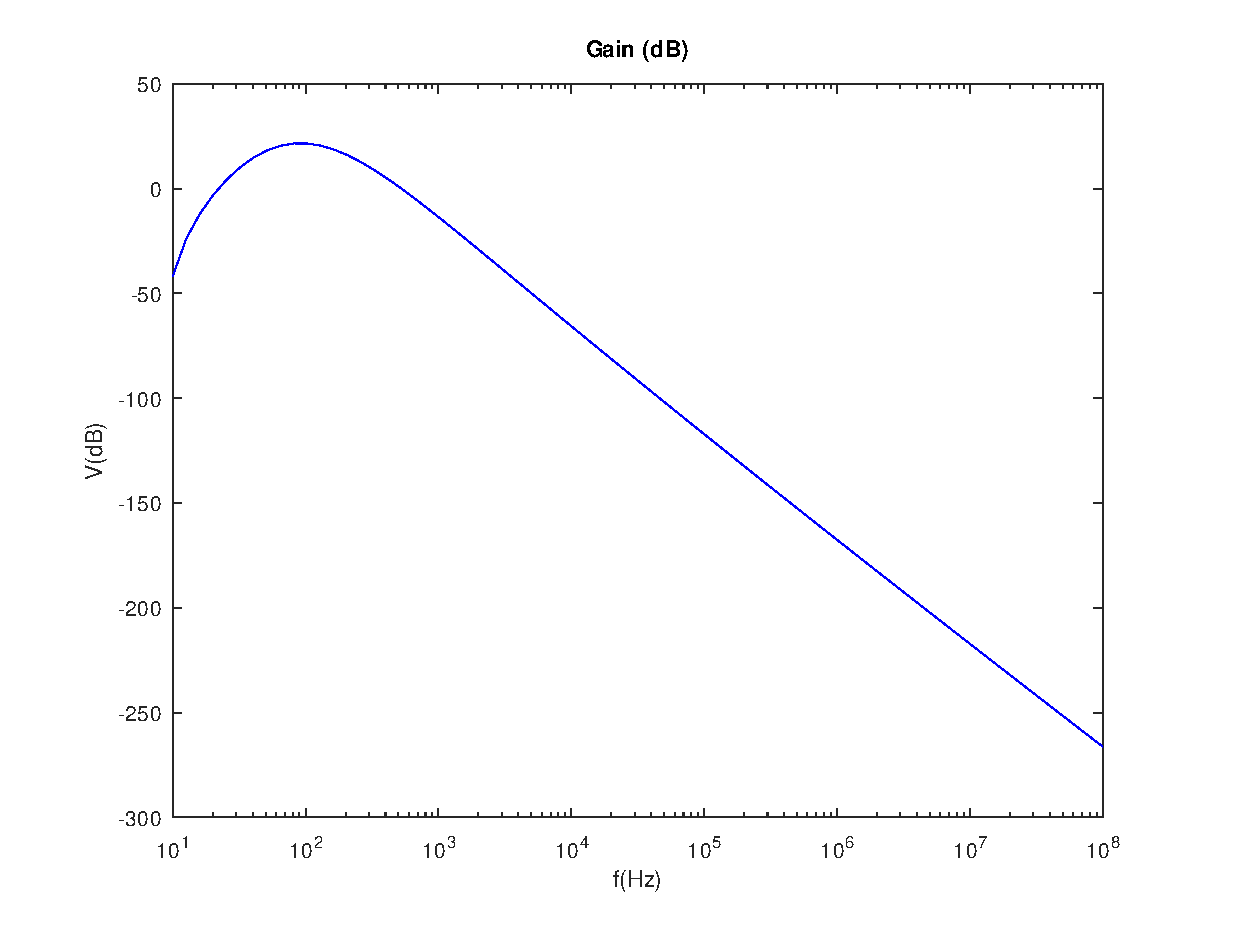
\includegraphics[width=0.8\linewidth]{t5dB.eps}

As such the central frequency is $81.855 Hz$, the gain at this frequency is $21.542 dB$ and the bandwidth is $143.57$.
These values are not consistent with the values given by simulation, however, they are consistent with the transfer function provided in the lab class:

\begin{equation}
    T(s)=\frac{R1*C1*s}{1+R1*C1*s}\cdot \frac{1+R3/R4}{1+R2*C2*s}
\end{equation}

As we can see in the plot below:

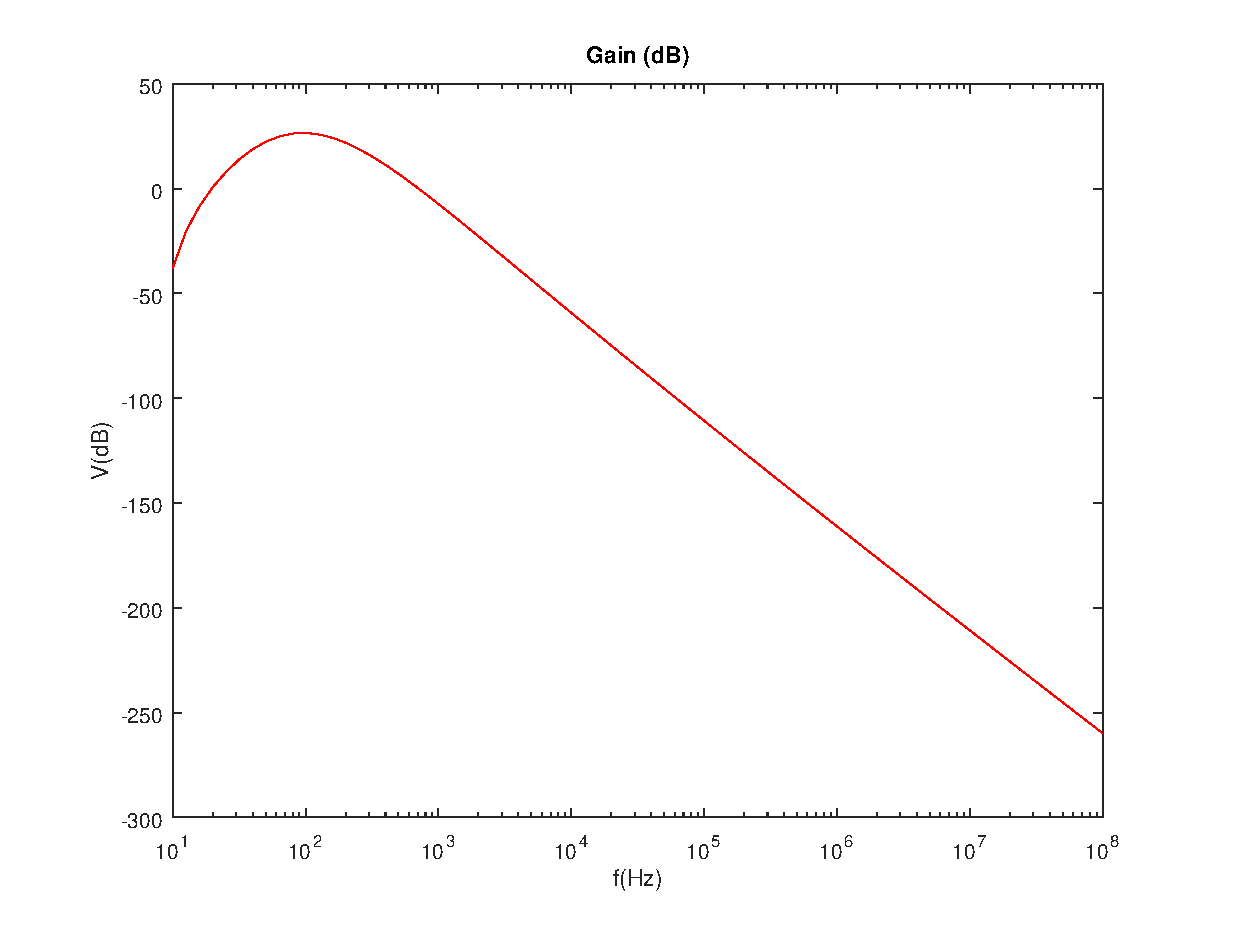
\includegraphics[width=0.8\linewidth]{teodB.eps}

The input and output impedances were also calculated yielding values of $1009.6 Ohm$ and $2.24\cdot 10^{-5} Ohm$ respectively.